\section{HASIL}

\subsection{Hasil Sementara}
Hasil sementara yang sudah dilakukan adalah mencoba penerapan CNN pada model yang mendeteksi citra wajah
sebagai pria atau wanita dengan menggunakan dataset dummy.
\begin{figure} [H] \centering
  % Nama dari file gambar yang diinputkan
  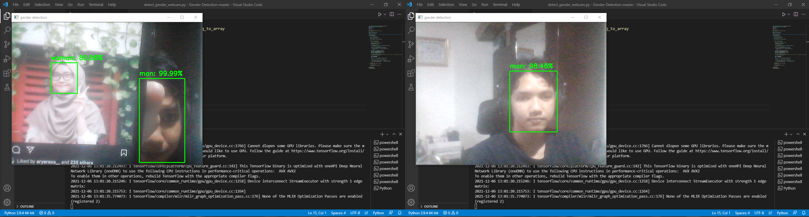
\includegraphics[scale=0.8]{gambar/HasilSementara.png}
  % Label referensi dari gambar yang diinputkan
  \label{fig:HasilSementara}
\end{figure}

\begin{center}
  % Keterangan gambar yang diinputkan
  Gambar 4.1 : Hasil sementara
\end{center}

\subsection{Hasil yang Diharapkan}
Hasil yang diharapkan dari Tugas Akhir ini adalah model yang dapat mendeteksi dan mengestimasi umur, 
gender dan etnik melalui fitur wajah manusia untuk mempermudah proses pengumpulan informasi.



\section{RENCANA KERJA}

% Ubah tabel berikut sesuai dengan isi dari rencana kerja
\newcommand{\w}{}
\newcommand{\G}{\cellcolor{gray}}
\begin{table}[h!]
  \begin{tabular}{|p{3.5cm}|c|c|c|c|c|c|c|c|c|c|c|c|c|c|c|c|}

    \hline
    \multirow{2}{*}{Kegiatan} & \multicolumn{16}{|c|}{Minggu} \\
    \cline{2-17} &
    1 & 2 & 3 & 4 & 5 & 6 & 7 & 8 & 9 & 10 & 11 & 12 & 13 & 14 & 15 & 16 \\
    \hline

    % Gunakan \G untuk mengisi sel dan \w untuk mengosongkan sel
    Pemorsesan Dataset &
    \G & \G & \w & \w & \w & \w & \w & \w & \w & \w & \w & \w & \w & \w & \w & \w \\
    \hline

    Pemilihan Model &
    \w & \w & \G & \G & \G & \G & \G & \w & \w & \w & \w & \w & \w & \w & \w & \w \\
    \hline

    Training dan Tuning Model &
    \w & \w & \w & \w & \G & \G & \G & \G & \G & \G & \G & \w & \w & \w & \w & \w \\
    \hline

    Pengujian dan Analisa &
    \w & \w & \w & \w & \w & \w & \w & \w & \w & \w & \w & \G & \G & \G & \w & \w \\
    \hline
    
    Pembuatan Laporan &
    \G & \G & \G & \G & \G & \G & \G & \G & \G & \G & \G & \G & \G & \G & \G & \G \\
    \hline

  \end{tabular}
\end{table}